\documentclass[a4paper,11pt]{article}

\usepackage[spanish]{babel}
\usepackage[T1]{fontenc}
\usepackage[utf8]{inputenc}
\usepackage{textcomp}
\usepackage{amsmath}
\usepackage{amsfonts}
\usepackage{amssymb}
\usepackage{fancyhdr}
\usepackage{anysize}
\usepackage{graphicx}

\begin{document}
\marginsize{2cm}{2cm}{2cm}{2cm}
\renewcommand\contentsname{Indice}
\renewcommand{\footrulewidth}{0.4pt}
\renewcommand{\headrulewidth}{0.4pt}

\pagestyle{empty}

\begin{figure}
  \centering
    
\includegraphics{logo.png}
\end{figure}

\vfill
\vspace{4cm}
\vspace{4cm}
\vspace{4cm}
\begin{center}
	\Huge{Diseño de la Clase Ahorcado}\\
	\Huge{Trabajo Práctico 2}\\
\end{center}
\vspace{4cm}


\begin{center}
	\begin{tabular}{|c|c|c|}
		\hline
		\textbf{Nombre y Apellido}  & \textbf{Padrón}\\
		\hline
		 Jose Paz & 91841   \\
		\hline
	\end{tabular}
\end{center}

\vfill 

\begin{flushleft}
	\Large{Docente: Andres Juarez}\\
	\Large{Cuatrimestre: Primero}\\
	\Large{Año: 2020}\\
\end{flushleft}


\newpage

\begin{figure}
  \centering
    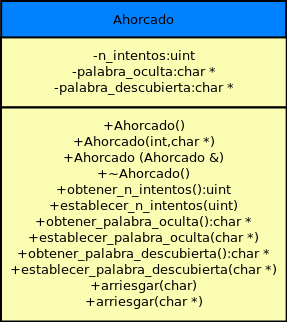
\includegraphics[width=0.5\textwidth]{Ahorcado_UML.png}
  \caption{Diseño UML de la clase Ahorcado}
  \label{fig:disenio}
\end{figure}

\end{document}
